\chapter{环境搭建与第一个圆盘场景}\label{ch:first}
\begin{notebox}
\textbf{本章目标}\quad 在主机 ROS 2 上编译两个小包，启动一个节点，在 RViz2 看见半径为 0.20 m 的圆盘。\\
\textbf{先修}\quad 会打开终端、编辑文本，读懂基本 C++ 变量和函数。
\end{notebox}

\section{先认识四个名字}
节点（node）是执行计算并收发消息的程序。话题（topic）是带名字和类型的数据通道，例如本章的 \code{/visualization/robot}。包（package）组织源码、依赖和安装规则。工作空间把多个包放到一起编译；它不是新的 ROS 发行版。

本章只有一个发布节点和一个可视化程序：
\begin{center}
\begin{tikzpicture}[node distance=28mm]
\node[draw=tealblue,fill=pale,rounded corners,inner sep=7pt] (a) {hello\_scene};
\node[draw=tealblue,fill=pale,rounded corners,inner sep=7pt,right=of a] (b) {RViz2};
\draw[-{Stealth},thick,tealblue] (a) -- node[above,font=\small] {Marker} (b);
\end{tikzpicture}
\end{center}
RViz2 显示收到的数据，不负责机器人动力学。本章圆盘是一个静态图形。

\section{确认主机环境}
本课程验证平台是 Ubuntu 26.04 和 ROS 2 Lyrical。已有主机不用重装。打开 bash，先运行：
\begin{lstlisting}[language=bash,numbers=none]
source /opt/ros/lyrical/setup.bash
printenv ROS_DISTRO
ros2 pkg prefix rviz2
colcon version-check --help
\end{lstlisting}
前三项应分别加载环境、输出 lyrical、找到 RViz2。最后一项只是检查 colcon 命令，后文构建才是实际工具链验收。

干净主机应先按
\href{https://github.com/ros2/ros2_documentation/blob/rolling/source/Get-Started/Installation/Ubuntu-Install-Debs.rst}{ROS 官方安装步骤}
配置 UTF-8、Universe 与 ros-apt-source。已配好软件源的 Ubuntu 26.04 可安装
\code{ros-lyrical-desktop}、\code{ros-dev-tools}、\code{libeigen3-dev}。
不要把其他 Ubuntu 版本与 Lyrical 的二进制包混用。

\begin{notebox}
Lyrical 的 ROS 接口按 C++20 编译；本课程独立几何和数学代码采用 C++17。读者不必先学习 concepts 等高级特性。ROS 的 Python 包使用系统 Python，构建时显式指定 \code{/usr/bin/python3}。
\end{notebox}

\section{构建并启动}
以下路径是当前主机仓库位置；换机器后改成自己的路径。每个新终端都要先加载主机环境，再加载课程工作空间。
\begin{lstlisting}[language=bash,numbers=none]
source /opt/ros/lyrical/setup.bash
cd /home/zdp/ForCodex/ros2_motion_planning_course/ros2_ws
colcon build --symlink-install --cmake-args \
  -DCMAKE_BUILD_TYPE=RelWithDebInfo \
  -DPython3_EXECUTABLE=/usr/bin/python3
source install/setup.bash
ros2 launch motion2d_bringup ch01.launch.py
\end{lstlisting}
\code{motion2d} 装算法和节点；\code{motion2d_bringup} 装配置、launch 与 RViz2 视图。
\code{--symlink-install} 方便开发时编辑配置。参数只在启动时读取，所以修改 YAML 后重启节点。

RViz2 应显示浅色背景、0.5 m 网格和原点的青色圆盘，Fixed Frame 为 map。无图形界面可加 \code{rviz:=false}；这不能替代图形验收。

\begin{figure}[htbp]
\centering
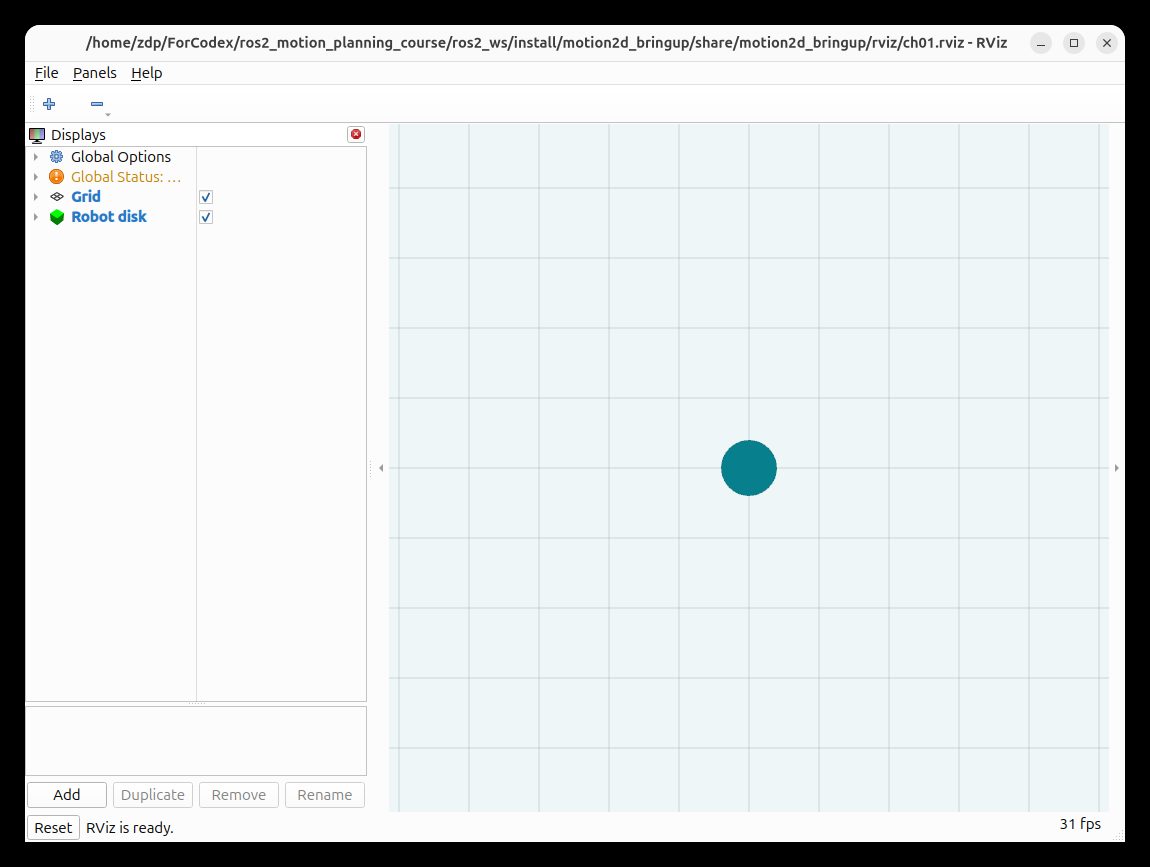
\includegraphics[width=.88\linewidth]{figures/ch01_rviz.png}
\caption{主机实际运行画面。圆盘直径为 0.40 m，小于一个 0.5 m 网格。}
\end{figure}
此时 Global Status 可能提示尚无 TF 数据，因为本章还没有发布坐标树。Marker 已直接在 map 帧中，所以仍可正确显示；下一章建立 TF 后该提示消失。

\section{圆盘为什么用直径？}
用一个很薄的 CYLINDER 表示圆盘。Marker 的 scale 是物体的完整尺寸，因此
\begin{equation}
d_x=d_y=2r,\qquad r=0.20\ \mathrm{m}\ \Rightarrow\ d_x=d_y=0.40\ \mathrm{m}.
\end{equation}
\code{scale.z=0.05} 只是显示厚度，后续平面碰撞只使用半径。单位四元数的 w 分量为 1；alpha 为 0 的图形完全透明。

下面直接读取实际源码的标记区域。修改代码后重新编译本书，摘录会同步更新：
\lstinputlisting[language=C++,linerange={marker_begin-marker_end},
  includerangemarker=false]{../ros2_ws/src/motion2d/src/nodes/hello_scene_node.cpp}

\section{发布一次，为什么晚启动也能看到？}
本节点使用 reliable + transient-local QoS，保留最后一条 Marker。RViz2 订阅同样配置持久性，晚启动时可取到保留的消息。节点退出后，不应假设消息仍会被保留。

第二个终端加载环境，进入工作空间后运行：
\begin{lstlisting}[language=bash,numbers=none]
ros2 topic echo /visualization/robot --once \
  --qos-durability transient_local
/usr/bin/python3 ../scripts/check_ch01.py
\end{lstlisting}
检查程序确实作为晚加入的订阅者接收消息，并核对帧、类型与默认尺寸。此时消息 stamp 用系统时间；下一章再引入仿真时钟。

\clearpage
\section{动手练习与验收}
\begin{enumerate}
\item \textbf{理解：}节点与话题的区别是什么？发布者先启动、RViz2 后启动时，为什么仍能收到圆盘？
\item \textbf{代码：}完成 \code{exercises/ch01/starter/marker_scale.hpp} 中的
\code{EXERCISE(ch01-1)}。检查方法、分级提示和独立参考答案位于同目录。
\item \textbf{实验：}在 \code{ch01.yaml} 中把半径改成 0.35 m、x 改为 1.0 m，重启。先预测消息和网格上的尺寸，再观察；检查默认配置前恢复参数。
\end{enumerate}
应看到直径 0.70 m、圆心 $(1,0)$ 的圆盘。若图形不见了，依次检查 Fixed Frame、话题、alpha 与 QoS。若找不到包，检查是否加载课程的 install 环境。

\subsection*{独立编译练习}
练习的输入是半径，输出是 Marker 的 x/y 尺寸。下面的 starter 故意保留一个需要你修改的返回值；它没有被链接到正式演示中。
\lstinputlisting[language=C++,numbers=none]{../exercises/ch01/starter/marker_scale.hpp}
从仓库根目录运行：
\begin{lstlisting}[language=bash,numbers=none]
g++ -std=c++17 -Wall -Wextra -Iexercises/ch01/starter \
  exercises/ch01/check.cpp -o /tmp/ch01_exercise
/tmp/ch01_exercise
\end{lstlisting}
未完成时检查输出 FAIL；改对后输出 PASS。检查包含两个半径，避免只为一个例子填写常数。若卡住，先看同目录的 hints，再读 solutions 的解释；把编译命令中的 starter 换成 solutions 即可验证参考解。

本章完成后，你应能解释图形由哪个节点发布、消息中哪些量决定尺寸，以及如何让另一个程序接收这条消息。
